\chapter{Risikomanagement}
	\label{risiken}
	
	\section{Übersicht über die Risiken}
		Um die Risiken im Projekt zu kennen und Massnahmen zu deren Minimierung umsetzen zu können, haben wir zu Beginn des Projekts eine Risikoanalyse erstellt und diese während des Projektverlaufs nach dem Abschluss jedes Meilensteins überarbeitet.
		In Abbildung~\ref{fig:RiskMatrix} und \ref{fig:RiskMatrixWeightedDamage} sind die im Kapitel~\ref{einzelneRisiken} detailliert aufgeführten Risiken in einer Übersicht dargestellt.
		
		\begin{figure}[H]
			\begin{minipage}[b]{\largeThird\linewidth}
				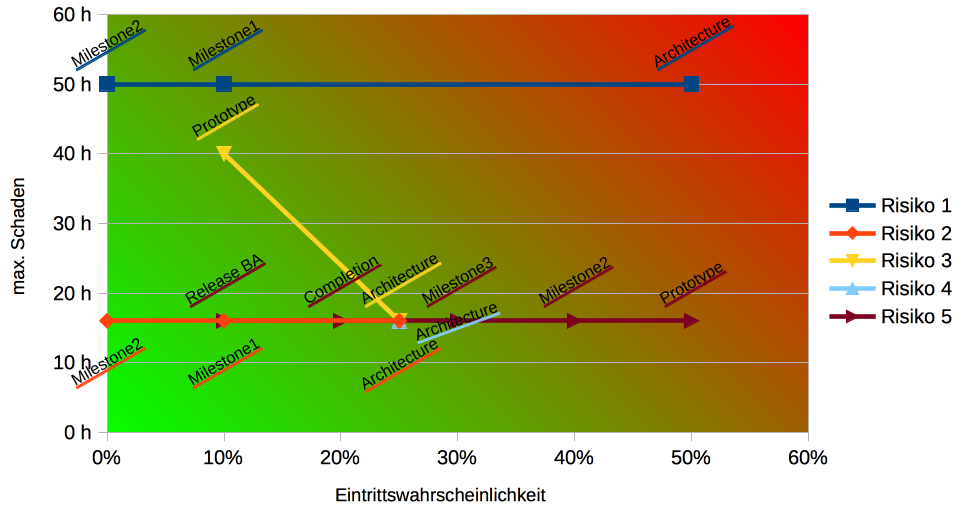
\includegraphics[width=0.9\textwidth]{projectPlan/media/img/risikomatrix.png}
				\centering
				\caption{Risikomatrix}
				\label{fig:RiskMatrix}
			\end{minipage}
			\begin{minipage}[b]{\smallThird\linewidth}
				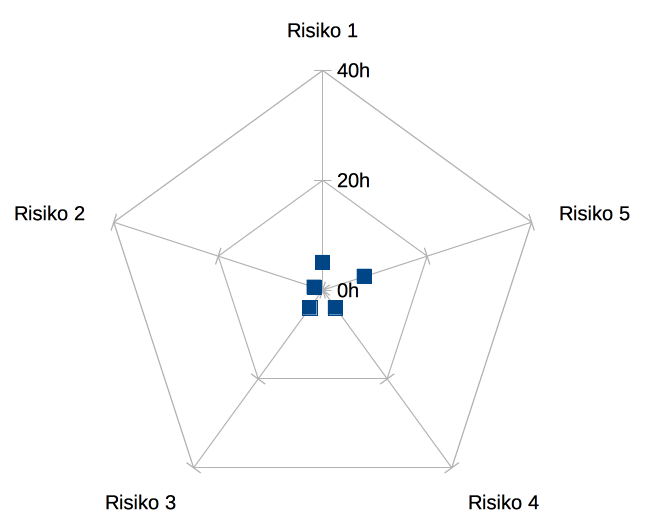
\includegraphics[width=0.9\textwidth]{projectPlan/media/img/risikomatrixGewichteterSchaden.png}
				\centering
				\caption{Gewichtete Schäden}
				\label{fig:RiskMatrixWeightedDamage}
			\end{minipage}
		\end{figure}
	
		Abbildung~\ref{fig:RiskMatrix} zeigt übersichtlich in Form eines X/Y-Diagramms welches Risiko wie wahrscheinlich ist (X-Achse) und wie gross der Schaden maximal bei einem Eintritt geschätzt wurde (Y-Achse).
		Abbildung~\ref{fig:RiskMatrixWeightedDamage} zeigt die gewichteten Schäden pro Risiko in Form eines Spiders.
		Die Gewichtung dabei ist die Multiplikation der Wahrscheinlichkeiten mit dem maximalen Schaden.
		
	Es ist deutlich zu sehen, dass das Risiko~1 dabei am kritischsten ist und dieses deshalb möglichst früh angegangen werden muss.
	Natürlich haben wir auch für die übrigen Risiken Massnahmen getroffen.
	Die für jedes Risiko getroffenen vorbeugenden Massnahmen sind im Kapitel~\ref{einzelneRisiken} direkt bei jedem Risiko selbst aufgeführt.
	

	\section{Einzelne Risiken}\label{einzelneRisiken}
		\newcounter{riskidcounter}
		
		\newcommand{\riskTable}[6]{
			%Die Spalten werden aufgeteilt auf dem goldenen Schnitt
			\noindent
			\refstepcounter{riskidcounter}
			\begin{tabular}{|p{\smallThird\textwidth} | p{\largeThird\textwidth} |}
				\hline	
				Risiko-ID 		& Risiko \theriskidcounter \\
				\hline
				Titel 			& #1 \\
				Beschreibung 		& #2 \\
				max. Schaden		& #3  \\
				Eintrittswahrscheinlichkeit & #4  \\
				Gewichteter Schaden	& #5  \\
				Vorbeugung/Massnahmen		& #6 \\
				\hline
			\end{tabular}
			\hspace{0.5cm}
			\newline	
		}
		
		\riskTable{Qualität der \cdar\ Schnittstelle}
		{Reicht die \cdar\ Schnittstelle nicht, bzw. stellt sie nicht genügend Informationen bereit, so muss die \cdar\ Server Applikation angepasst werden.}
		{50h}{0.5}{25h}
		{Eignung der Schnittstelle durch den Prototyp abklären.}
		
		\riskTable{Einarbeitung Play Framework}
		{Die Einarbeitung des Teammitglieds, welches das Play Framework noch nicht kennt, dauert länger als angenommen.}
		{16h}{0.25}{4h}
		{Rechtzeitiges Einarbeiten ins Framework}
		
		\riskTable{Mapping Complexity}
		{Die Abbildung des Metamappings ist wesentlich komplexer als angenommen.}
		{40h}{0.1}{8h}
		{Minimales Mapping bereits im Prototyp umsetzen um Komplexität abschätzen zu können. Mapping Features priorisieren, die Kernfunktionalität abdecken, Nebenfunktionalität weglassen.}

		\riskTable{Schnittstelleneinheitlichkeit}
		{Die Schnittstellen der gängigen Projektmanagementsysteme sind zu unterschiedlich, als das sie über einen Adapter mit einer Konfiguration abgedeckt werden können.}
		{16h}{0.25}{4h}
		{Bereits während der Prototypenphase verschiedene Schnittstellen berücksichtigen.}

		\riskTable{Ausfall Infrastruktur}
		{Die Infrastruktur des Projekts fällt aus.}
		{16h}{0.5}{8h}
		{Regelmässig Backups der kritischen Daten erstellen.}
